A partir de los datos de los casos penales, pudimos construir la red de \textit{Grupos de Pertenencia}. En esta red se eliminan los nodos de aquellas personas cuyos roles no sean referidos a actores delictivos, como ser denunciantes, víctimas o damnificados. 
Una visualización de los datos puede verse en la Figura \ref{fig:grafoTop10}.
Al analizar la composición de la red obtenida podemos observar las relaciones que existen entre los nodos y como se "equilibra" el grafo, haciendo que aquellos nodos con pocas o nulas relaciones queden en la periferia de la gráfica. Sumado a ello también es apreciable la medida de centralidad de aquellos nodos que son rodeados por sus relacionados. 
%Una aproximación para denotar la medida de centralidad puede verse reflejada 
En la Figura \ref{fig:grafoTop10} se visualizan sólo las 10 personas con más Casos y sus grupos de pertenencia. Claramente esos 10 nodos principales quedan rodeados de sus grupos de pertenencia y se pueden observar transitividades entre ellos a través de nodos que conforman parte del grupo de pertenencia de más de un nodo principal.
%\vspace{-15pt}
\begin{figure}
	\centering
	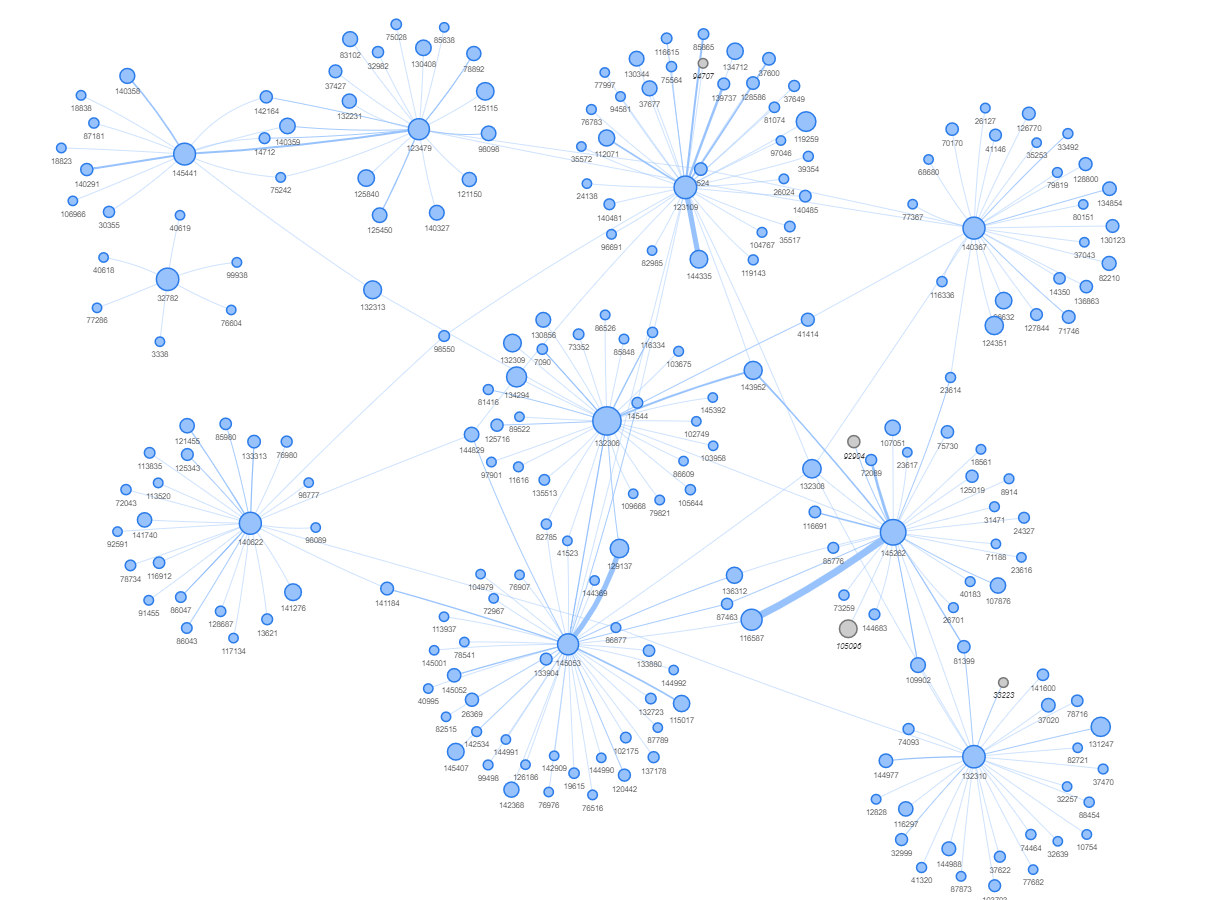
\includegraphics[width=0.5\linewidth]{grafo-10-completo.png}
	\caption{10 personas con más casos en Coirón, con sus relaciones} 
	\label{fig:grafoTop10}
\end{figure}
%\vspace{-15pt}